
\section{I - Introduction}
\begin{frame}{I - Introduction}
	\begin{block}{Présentation du modèle du perceptron}
		C'est  en 1943, que McCulloch et Pitts introduisent le modèle du perceptron.  \\
		Ce modèle est basé sur le fonctionnement du neurone humain.
	\end{block}
	\begin{figure}
		\centering
		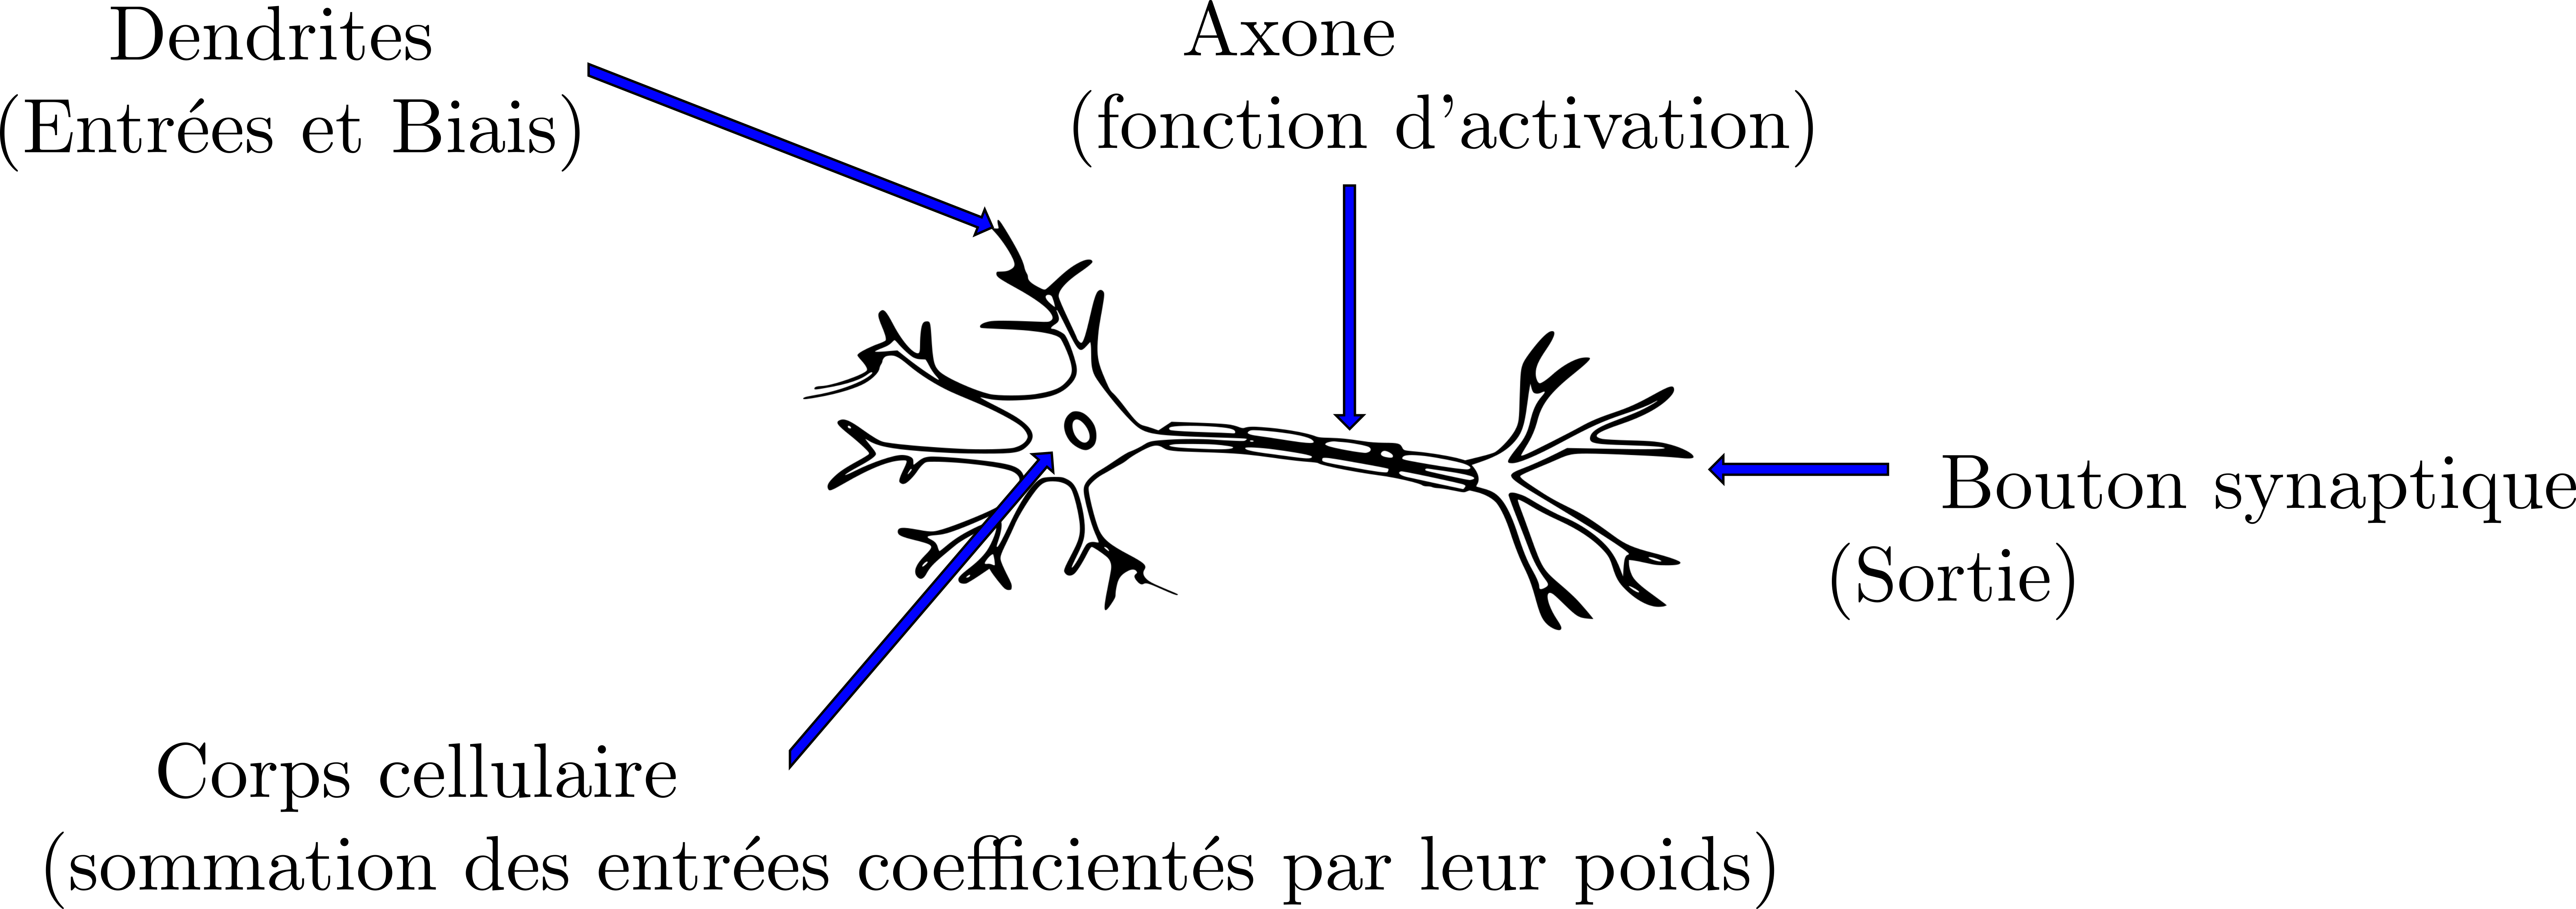
\includegraphics[width=\textwidth]{2-Neurone.png}
		\caption{Schéma d'un neurone humain}
	\end{figure}
\end{frame}


\begin{frame}{I - Le perceptron}
	\begin{figure}
		\centering
		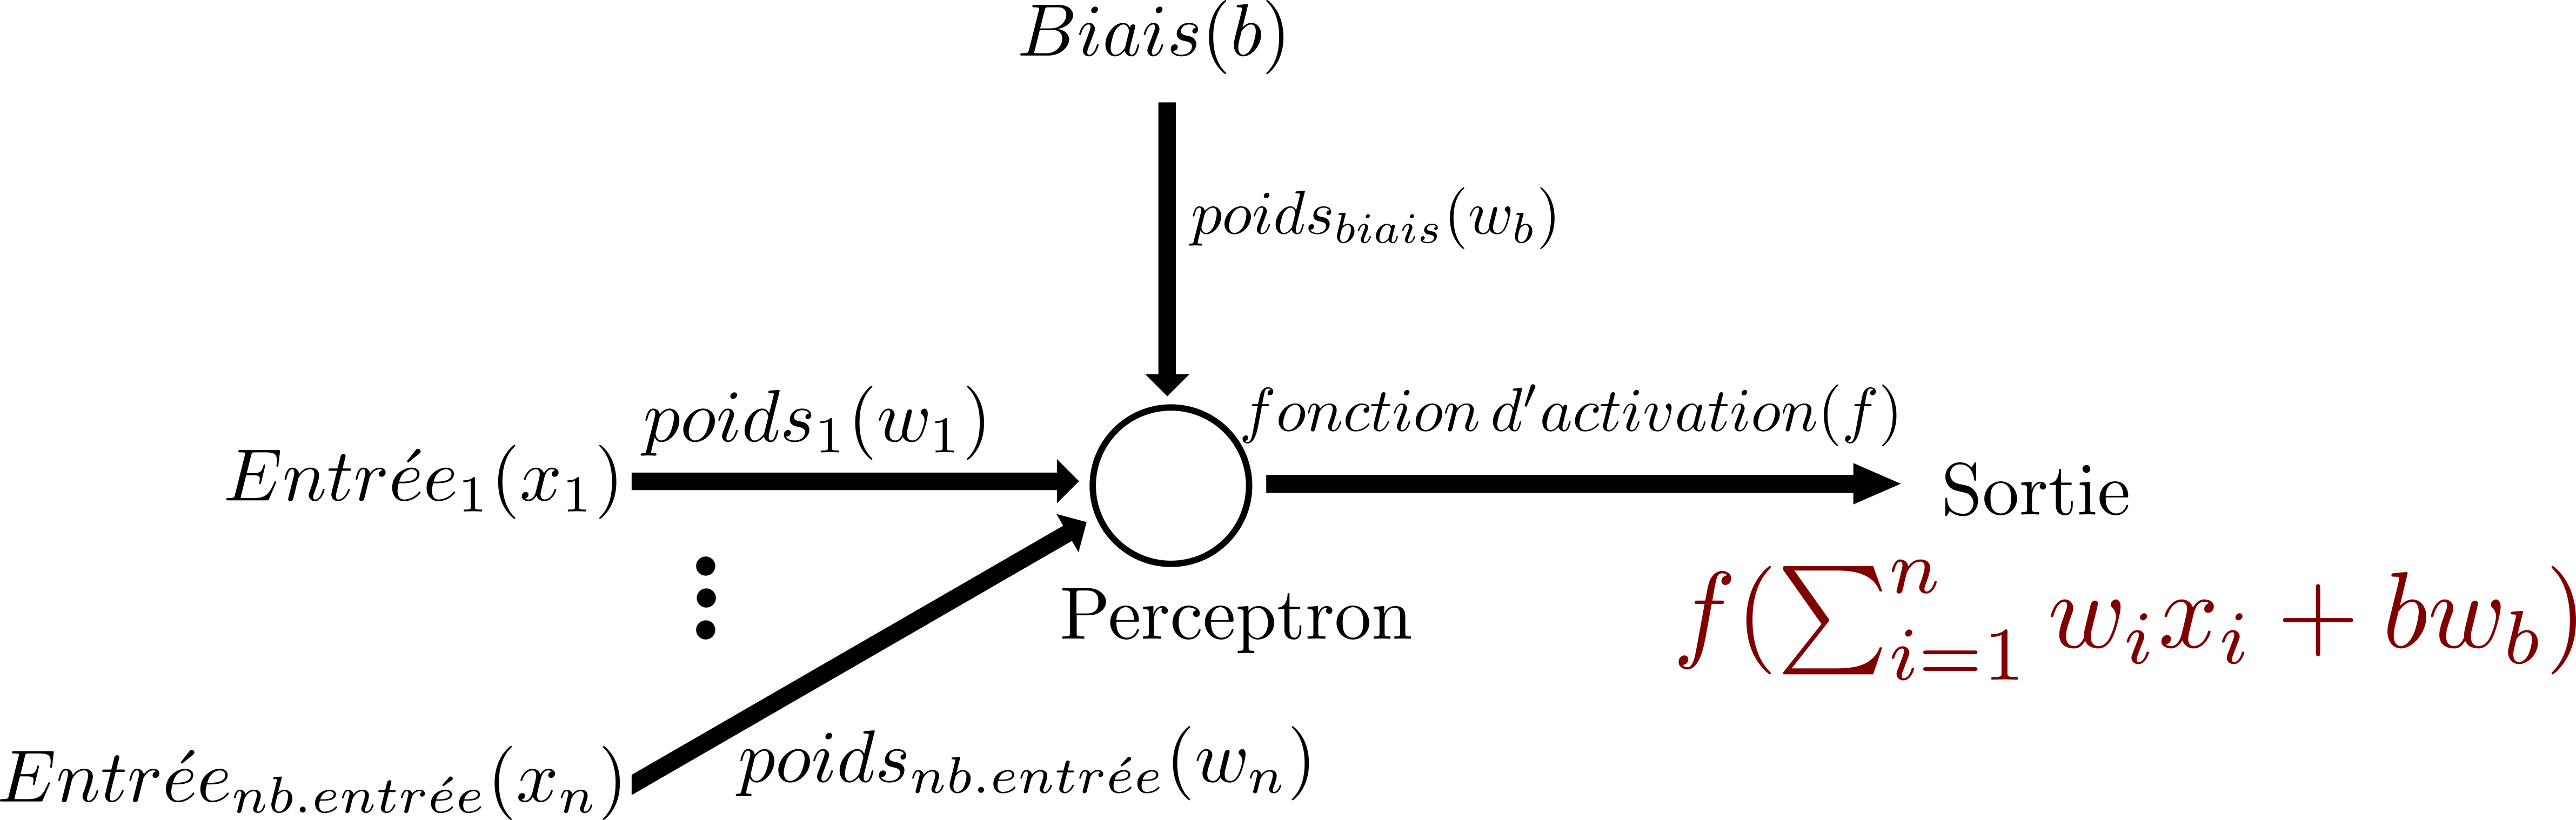
\includegraphics[width=\textwidth]{1-Perceptron.png}
		\caption{Schéma d'un perceptron}
	\end{figure}
\end{frame}


\begin{frame}{I - Représentation informatique}
	\begin{columns}
		\begin{column}[]{0.4\textwidth}
			\begin{center}
				$
					f
					\left(
					\begin{pmatrix}
						x_1 & \ldots & x_n & b
					\end{pmatrix}
					\times
					\begin{pmatrix}
						w_1    \\
						\vdots \\
						w_n    \\
						w_b
					\end{pmatrix}
					\right)
				$ \\
				\openup 1em
				La complexité est en $O(n)$
			\end{center}
		\end{column}
		\begin{column}[]{0.5\textwidth}
			\lstinputlisting[language=Python, firstline=15]{0-representation.py}
		\end{column}
	\end{columns}
	\caption{Représentation informatique du perceptron}
\end{frame}